\documentclass[main.tex]{subfiles} % Subfile-Class


% ============================================================================== %
%                            Subfile document                                    %
% ============================================================================== %

\begin{document}

% Template

\subsubsection{Abstandssensoren}~\label{appendix:Abstandssensoren_Kapitel}

Wie die Konzeption der Abstandssensoren (siehe
Anhang~\ref{appendix:Hinderniserkennung}) gezeigt hat, wird die Umfelderkennung
im ersten Prototypen redundant ausgeführt und im Folgemodul weiter verfeinert.

Das in PREN1 erarbeitete Konzept sieht vor, den Abstand zu potentiellen Pylonen
mittels LIDAR über die Hindernisse hinweg zu erfassen. Sind diese näher als 2 m
- ist die betrachtete Strecke wahrscheinlich nicht befahrbar. Ein zweiter
Abstandssensor, der mit Ultraschall arbeitet, erkennt Hindernisse, die näher
als 0,5 m sind. Dadurch kann das Fahrzeug rechtzeitig abgebremst werden. Wird
die am Greifer positionierte Lichtschranke ausgelöst, kann mit Sicherheit davon
ausgegangen werden, dass das Fahrzeug nun beginnen kann und soll, das Hindernis
zu greifen und umzupositionieren.

Die Funktion der Lichtschranke könnte auch vom Ultraschallsensor übernommen
werden, was im Folgemodul weiter untersucht wird. Ebenso befindet sich auf dem
Fahrzeug eine Kamera, die die vorhandenen Wegpunkte analysieren kann. Mit
dieser Kamera könnten auch Hindernisse erkannt werden, dies wird aber ebenfalls
erst im Folgemodul weiter untersucht, wenn ein erster Prototyp aufgebaut ist.

\paragraph{Fazit} 
Das in Abbildung~\ref{fig:Konzept_Hinderniserkennung} gezeigte Konzept stellt
den aktuellen Stand der Entwicklung dar und ist so für den ersten Aufbau
eingeplant.

\begin{figure}[H]
    \centering
    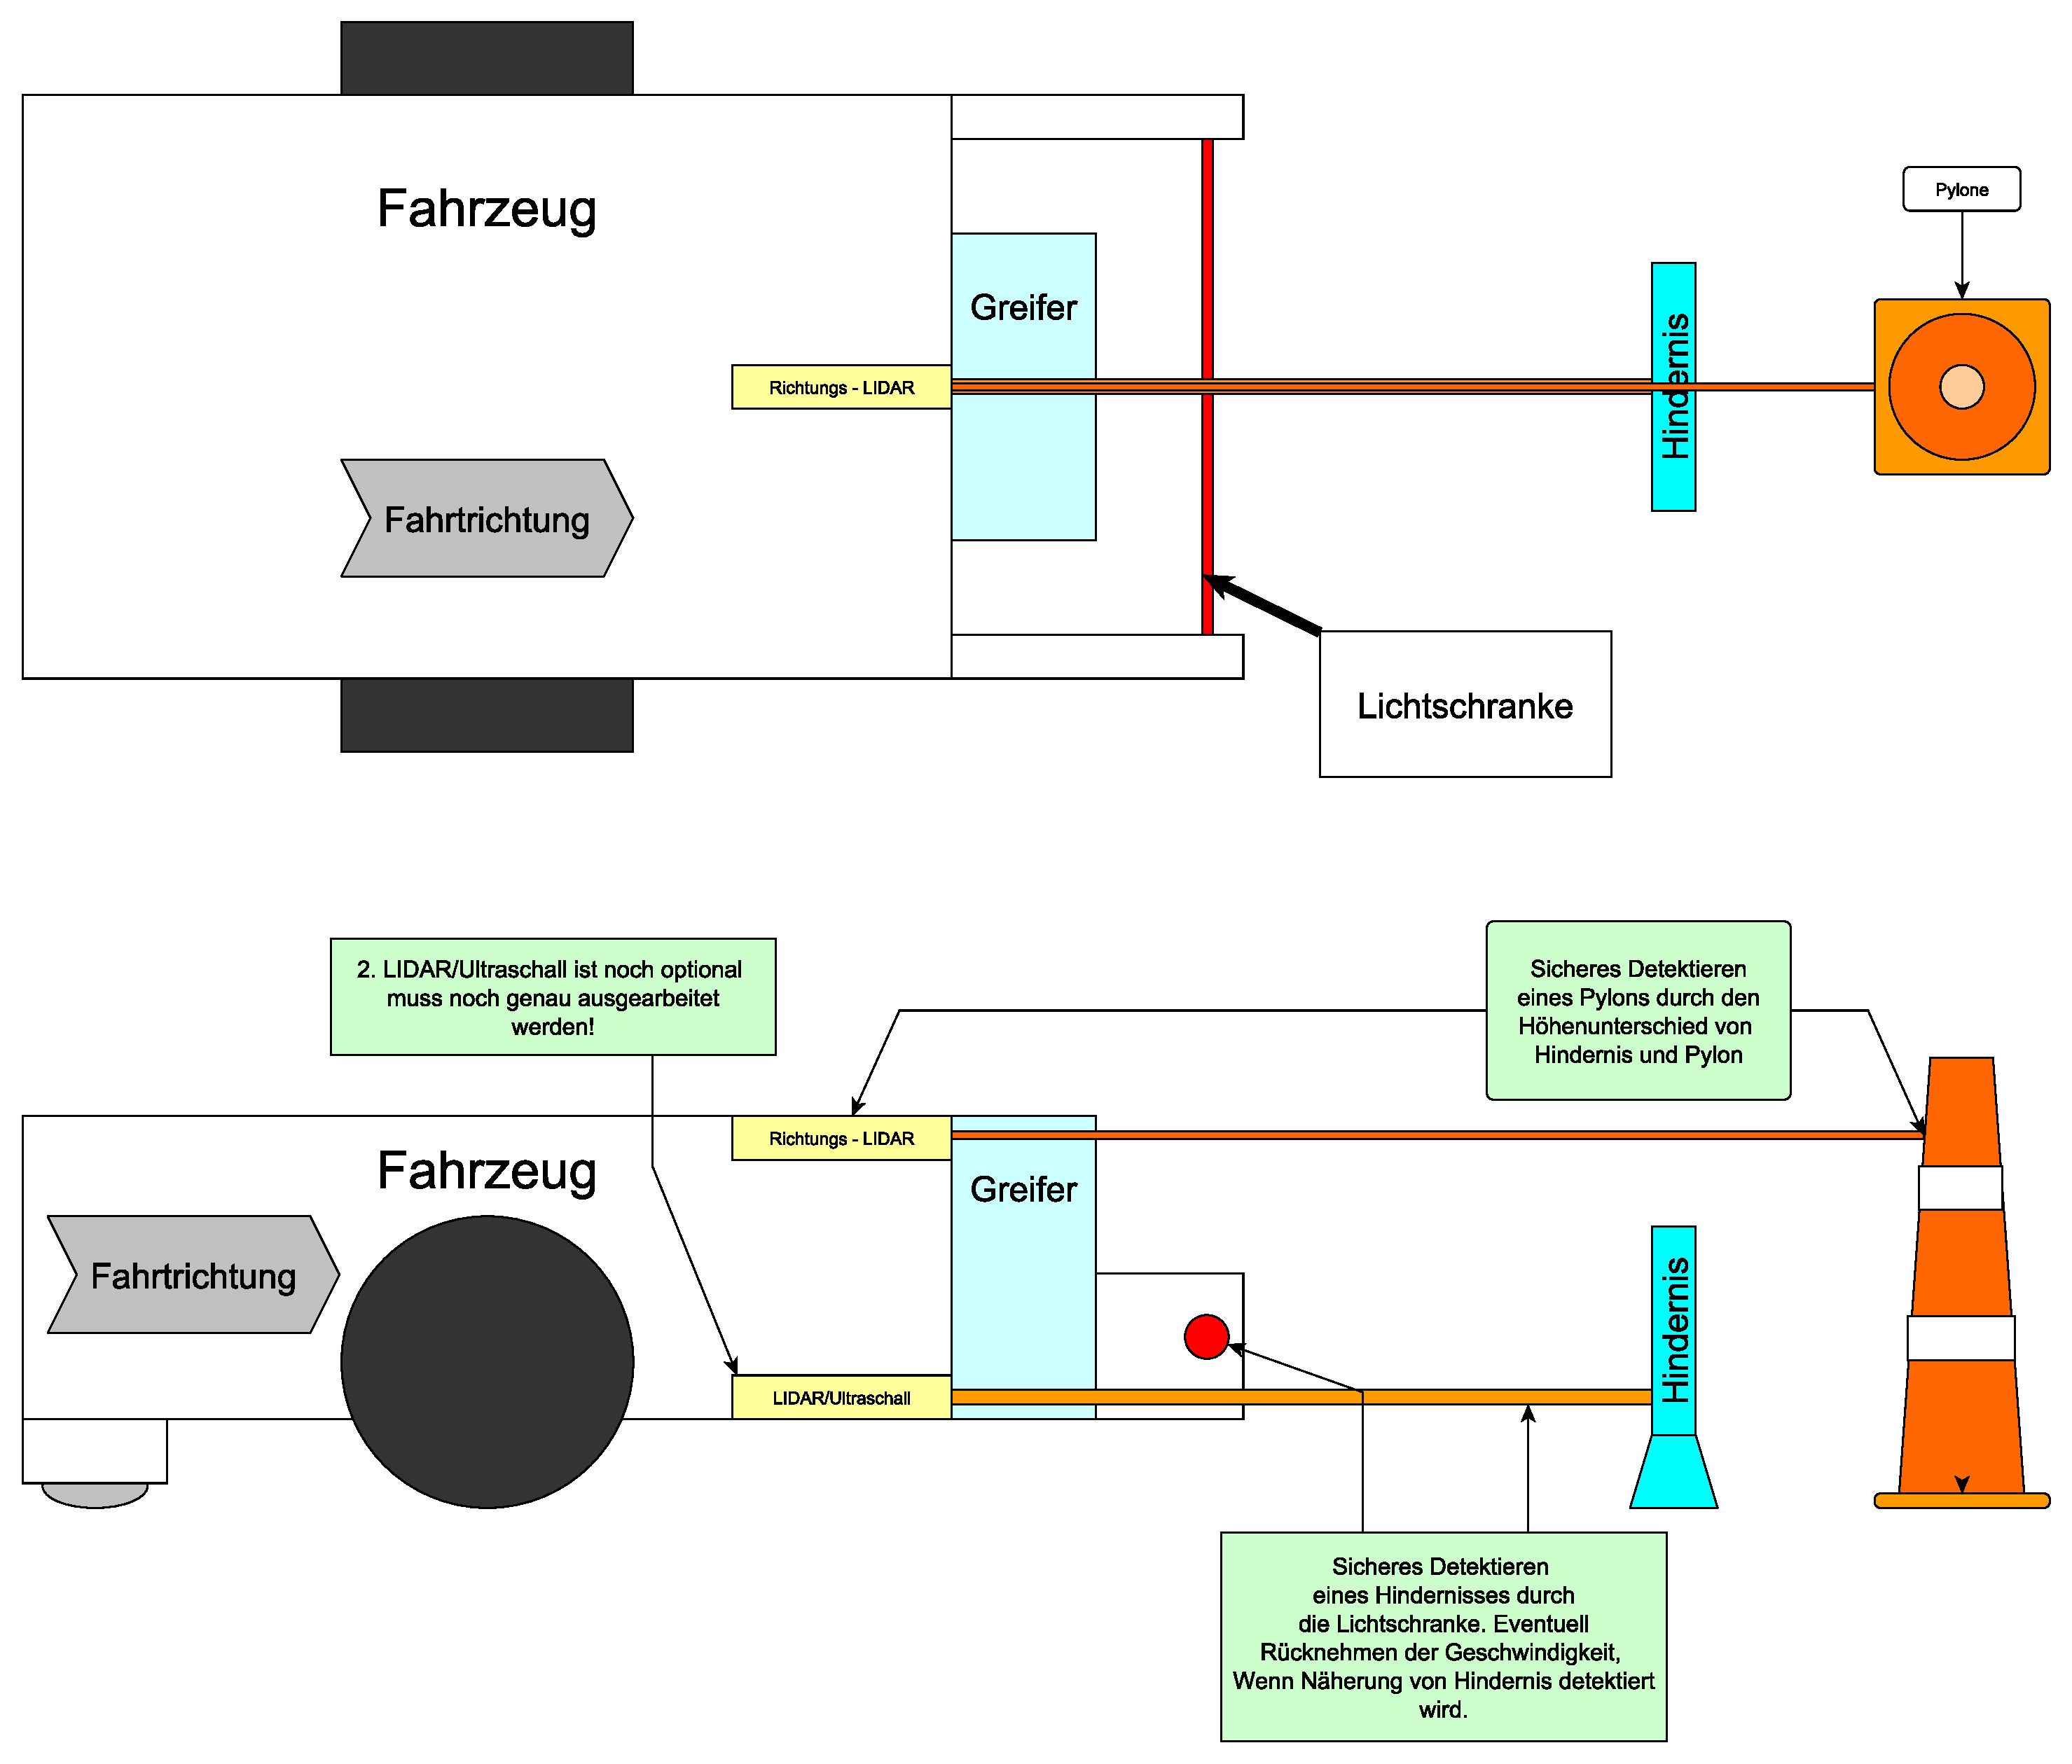
\includegraphics[width=0.75\linewidth]{./fig_Abstandssensor/Konzept_Hinderniserkennung.pdf}
    \caption{Konzept Hinderniserkennung}~\label{fig:Konzept_Hinderniserkennung}
\end{figure}

\paragraph{Eingesetzte Sensoren}
Verwendet wird der Ultraschallsensor \textit{HC-SR04}, sowie der
Richtungs-LIDAR \textit{TFLuna}.

\end{document}
